\documentclass[12pt,letterpaper]{article}
\usepackage[utf8]{inputenc}
\usepackage[spanish]{babel}
\usepackage{graphicx}
\usepackage[left=2cm,right=2cm,top=2cm,bottom=2cm]{geometry}
\usepackage{graphicx} % figuras
% \usepackage{subfigure} % subfiguras
\usepackage{float} % para usar [H]
\usepackage{amsmath}
%\usepackage{txfonts}
\usepackage{stackrel} 
\usepackage{multirow}
\usepackage{enumerate} % enumerados
\renewcommand{\labelitemi}{$-$}
\renewcommand{\labelitemii}{$\cdot$}
% \author{}
% \title{Caratula}
\begin{document}

% Fancy Header and Footer
% \usepackage{fancyhdr}
% \pagestyle{fancy}
% \cfoot{}
% \rfoot{\thepage}
%

% \usepackage[hidelinks]{hyperref} % CREA HYPERVINCULOS EN INDICE

% \author{}
\title{Caratula}

\begin{titlepage}
\begin{center}
\large{UNERSIDAD PRIVADA DE TACNA}\\
\vspace*{-0.025in}
\begin{figure}[htb]
\begin{center}

\includegraphics[width=8cm]{./Imagenes/logo}
\end{center}
\end{figure}
\vspace*{0.15in}
ESCUELA PROFESIONAL DE INGENIERIA DE SISTEMAS  \\

\vspace*{0.5in}
\begin{large}
TITULO:\\
\end{large}

\vspace*{0.1in}
\begin{Large}
\textbf{INFORME DE LABORATORIO No 02} \\
\end{Large}

\vspace*{0.3in}
\begin{Large}
\textbf{CURSO:} \\
\end{Large}

\vspace*{0.1in}
\begin{large}
INTELIGENCIA DE NEGOCIOS\\
\end{large}

\vspace*{0.3in}
\begin{Large}
\textbf{DOCENTE(ING):} \\
\end{Large}

\vspace*{0.1in}
\begin{large}
 Patrick Cuadros Quiroga\\
\end{large}

\vspace*{0.2in}
\vspace*{0.1in}
\begin{large}
Alumno: \\
\begin{flushleft}
Guimer Senon Coaquira Coaquira	\hfill	(2015053226) \\
\end{flushleft}
\end{large}
\end{center}

\end{titlepage}


\tableofcontents % INDICE
\thispagestyle{empty} % INDICE SIN NUMERO
\newpage
\setcounter{page}{1} % REINICIAR CONTADOR DE PAGINAS DESPUES DEL INDICE
\begin{center}
\vspace*{0.1in}
\begin{Large}
\textbf{PRACTICA DE LABORATORIO N° 02:} \\
\textbf{(Modelando Datos en Power BI)} \\
\end{Large}
\end{center}
\begin{document}
\section{OBJETIVO:}
\item{
Desarrollar el Informe de Labratorio 02 de Modelando Datos en Power BI}
\section{REQUERIMIENTOS}
\begin{itemize}

- Conocimientos básicos de administración de base de datos Microsoft   SQL Server.
\\- Conocimientos básicos de SQL.
\\- Microsoft SQL Server 2016 o superior
\\- Base de datos AdventureWorks2016 o superior
\\- Power BI Desktop.
\\- Tener una cuenta Microsoft registrada en el Portal de Power Bi.
\end{itemize}
\section{CONSIDERACIONES INICIALES}
\item{Generar una carpeta o directorio Power BI en un lugar accesible para guardar los resultados de la práctica.}\\

\section{DESARROLLO}
\newpage
\subsection{IMAGEN Nº01:}
\begin{itemize}
Ingresar a Power BI Desktop, en el cuadro de dialogo Obtener Datos (Get Data), asegurarse que Excel esta seleccionado y hacer click en Conectar (Connect), buscar el archivo Adventure Works Sales Data.xlsx y hacer click en Cargar (Load).

\end{itemize} 

\begin{figure}[httb]
\begin{center}
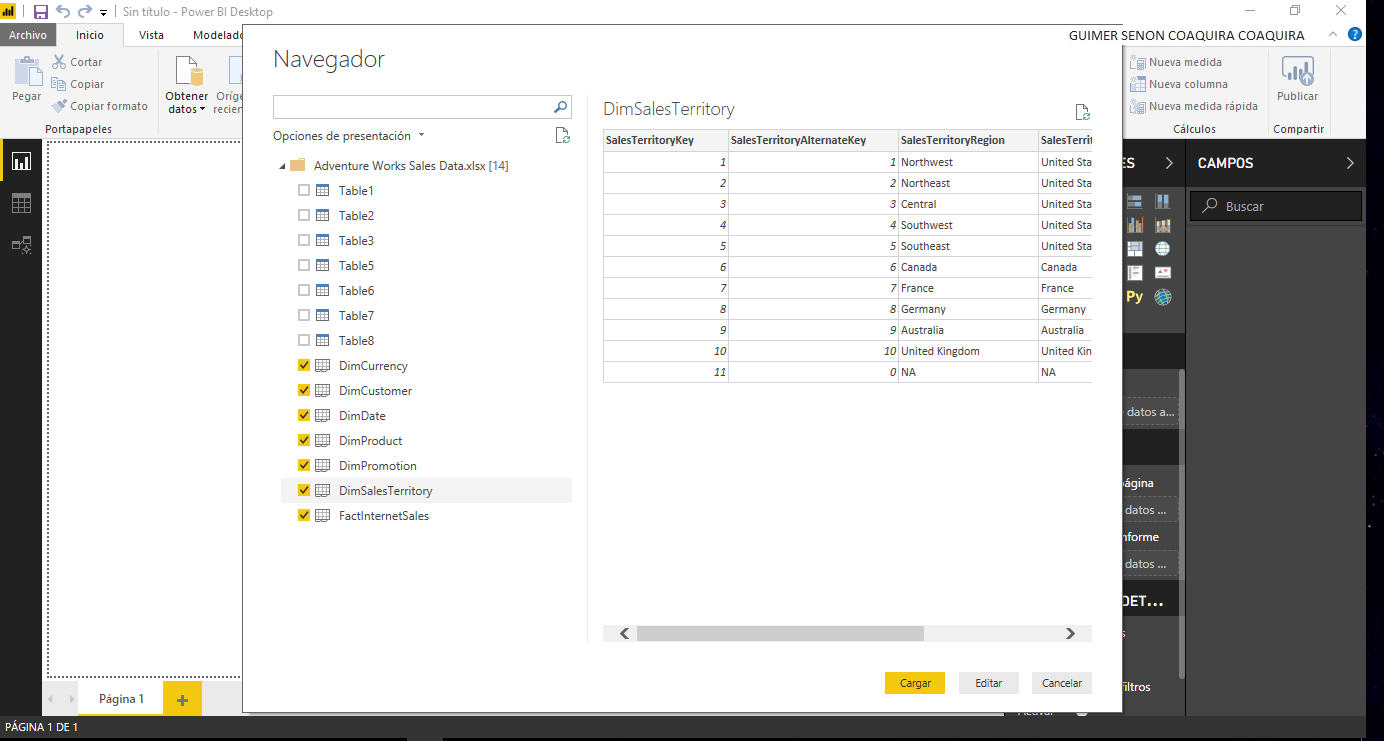
\includegraphics[width=13cm]{./Imagenes/Captura01}
\end{center}
\end{figure}

\subsection{IMAGEN Nº02:}
\begin{itemize}
En el cuadro de Administrar relaciones (Manage Relationships) realizar las configuraciones indicadas 
\end{itemize} 

\begin{figure}[httb]
\begin{center}
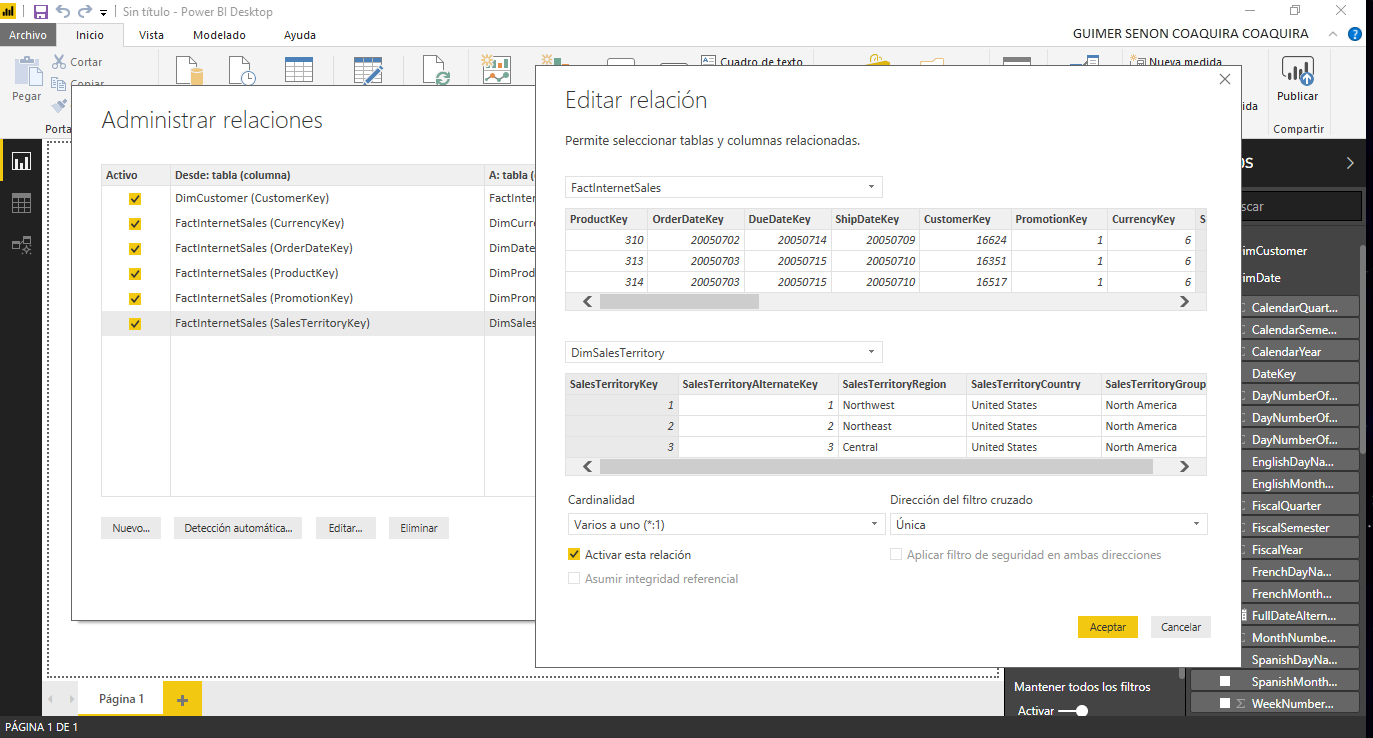
\includegraphics[width=13cm]{./Imagenes/Captura02}
\end{center}
\end{figure}
\newpage
\subsection{IMAGEN Nº03:}
\begin{itemize}
Abrir el archivo Adventure Works Product Categories.xlsx
\end{itemize} 

\begin{figure}[httb]
\begin{center}
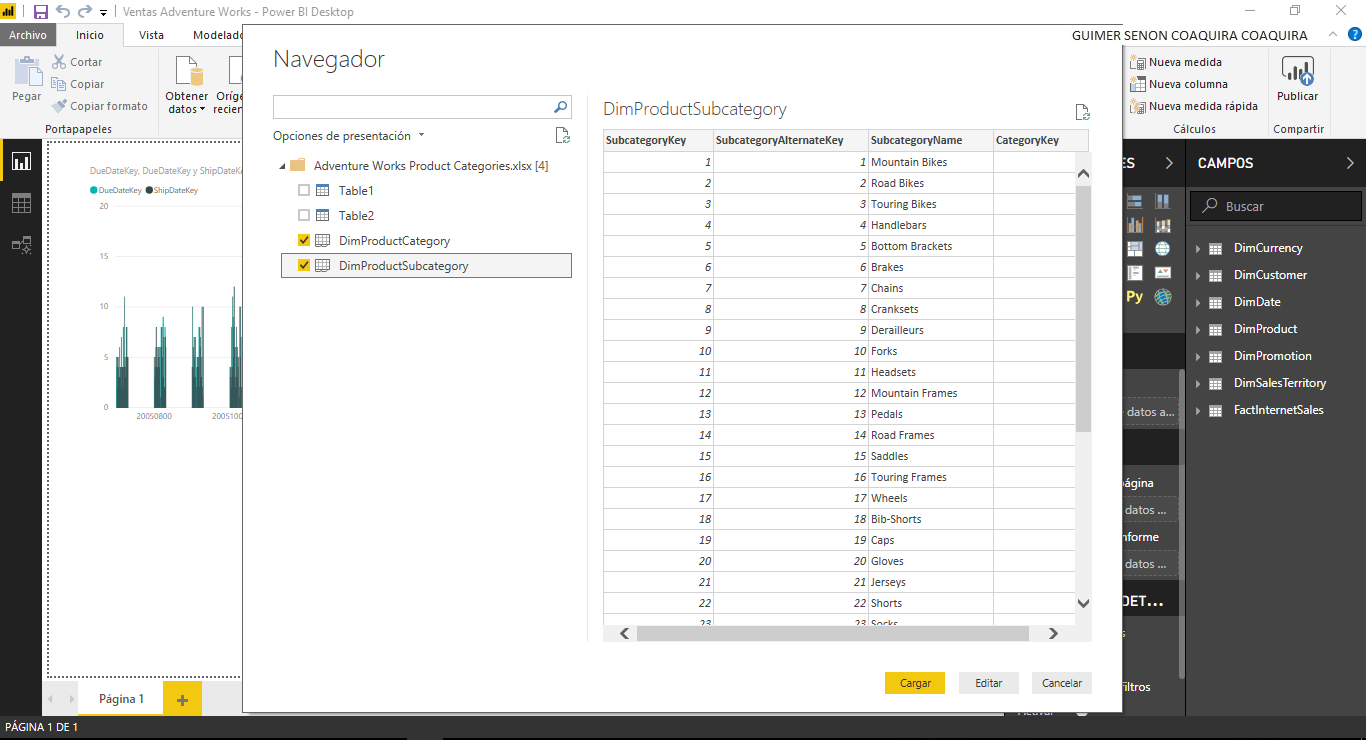
\includegraphics[width=13cm]{./Imagenes/Captura04}
\end{center}
\end{figure}



\subsection{IMAGEN Nº04:}
\begin{itemize}
En el panel Campos, haga clic en DimCustomer,en la cinta Modelado, en el grupo Cálculos, haga clic en Nueva columna.En la barra de fórmulas, resalte Columna = y escriba:
IncomeStatus = IF (DimCustomer[YearlyIncome] < 25000, "Lower Income",
IF (AND(DimCustomer[YearlyIncome] >= 25000, DimCustomer[YearlyIncome] < 60000),
"Middle Income",
IF (AND(DimCustomer[YearlyIncome] >= 60000, DimCustomer[YearlyIncome] < 100000),
"Higher Income",
IF (DimCustomer[YearlyIncome] >= 100000, "Very High Income", "Other")))) y finalmente presione Enter.
\end{itemize}

\begin{figure}[httb]
\begin{center}
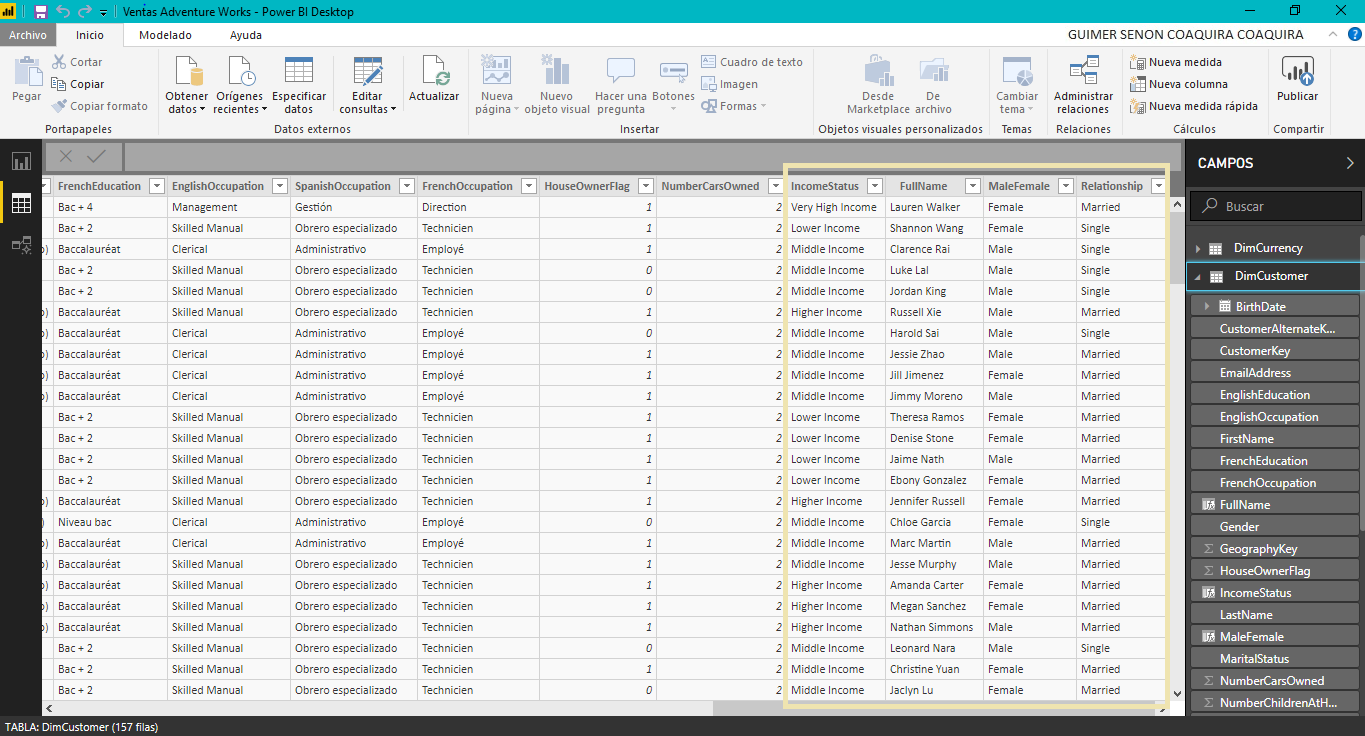
\includegraphics[width=13cm]{./Imagenes/Captura06}
\end{center}
\end{figure}

\newpage
\subsection{IMAGEN Nº05:}
\begin{itemize}
En el panel Campos, haga clic en FactInternetSales.En la cinta Modelado, en el grupo Cálculos, haga clic en Nueva columna y realizar la siguiente operacion:
Profit = CURRENCY(FactInternetSales[UnitPrice] -
FactInternetSales[ProductStandardCost])
\end{itemize}

\begin{figure}[httb]
\begin{center}
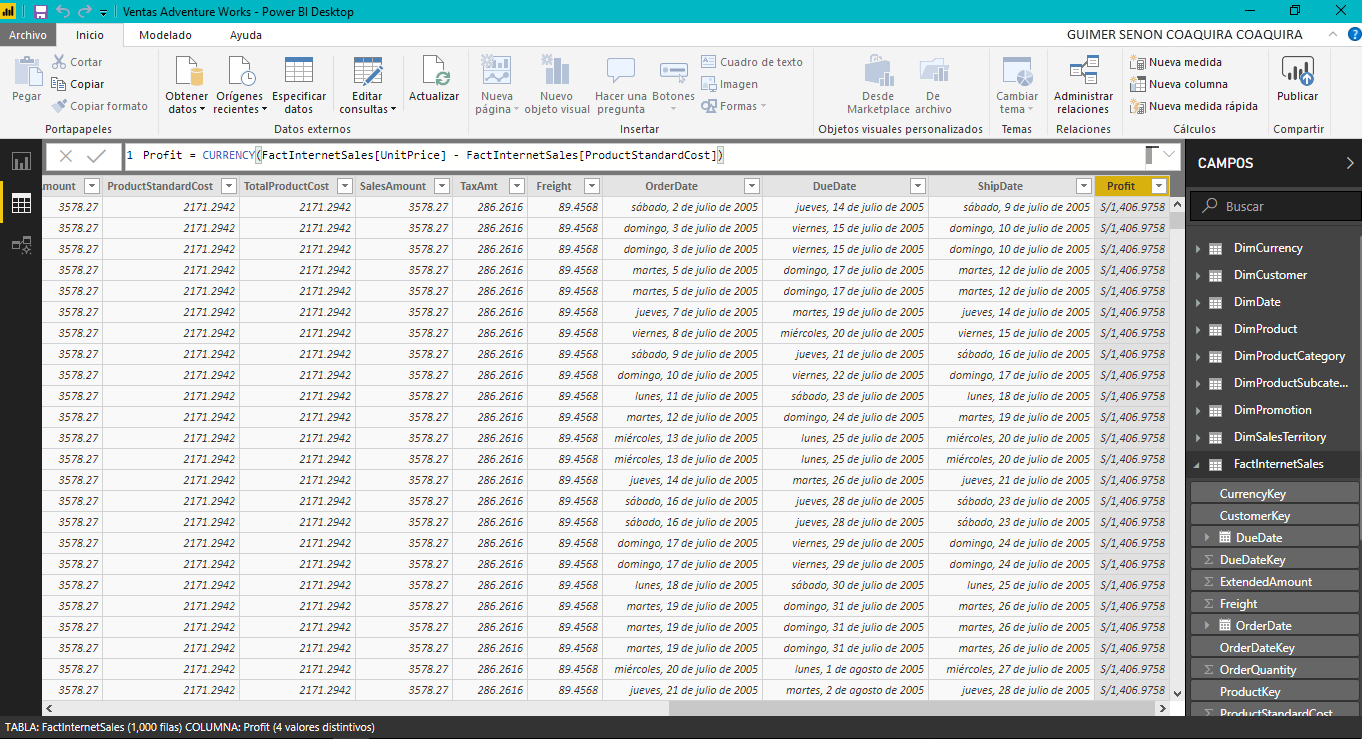
\includegraphics[width=13cm]{./Imagenes/Captura08}
\end{center}
\end{figure}


\end{document}

